\chapter[Our Framework at Work on the iTrust SWaT System]{Our Framework at Work: Reverse Engineering of the iTrust SWaT System}
\label{application}
\linenumbers

\lettrine{I}{n this} chapter, our main objective is to apply the framework and methodology introduced in Chapter \ref{chap:proposal} to the case study of the iTrust SWaT system, as illustrated in Chapter \ref{casestudy}. The purpose of this analysis is to assess the effectiveness and potential of the proposed framework within the context of a system that closely replicates a real-world water treatment plant, albeit on a smaller scale.

\bigskip
Due to the complexity of the system and the limited space available in this thesis, we will not conduct a comprehensive analysis and reverse engineering of the entire system. Instead, we will focus on specific parts for analysis. We leave it to the reader or those interested in utilizing the proposed methodology and framework to complete the analysis, should they choose to do so.

By focusing on selective components and leaving room for further exploration, we strike a balance between providing valuable insights and acknowledging the potential for additional research. This approach empowers the reader and interested individuals to explore the iTrust SWaT system further and leverage the proposed methodology and framework for a more comprehensive analysis.

\section{Preliminary Operations}
\label{sec:6_preliminar_operations}
Prior to beginning the actual analysis, several preliminary manual operations need to be conducted on the physical process dataset utilized as a case study, specifically the SWaT system dataset for the year 2015 as outlined in Section \ref{subsec:5_2015_datasets}. To simulate the data-capture process performed by Ceccato et al. using their scanning tool, the original dataset in XLSX format (proprietary to Microsoft Excel) was divided into multiple datasets in CSV format. Each of these datasets corresponds to the individual stages of the SWaT system and contains the respective registers. These resulting files were then saved in the directory specified by the \texttt{raw\_dataset\_directory} directive in the framework configuration file, \textit{config.ini}, ready to be used in the pre-processing phase.
Furthermore, the headers were manually renamed by adding a prefix from \texttt{P1\_} to \texttt{P6\_} to each register's name. This prefix indicates the stages, ensuring that each register is easily identifiable and linked to its corresponding stage.

\section{Planning the Analysis Strategy}
\label{sec:6_analysis_strategy}
The complexity of the system being analyzed necessitates the adoption of a deliberate strategy for the analysis. It is not feasible to rely on trial and error or attempt every possible combination between stages. The former approach may overlook crucial relationships between PLCs or between registers, while the latter may result in excessive and unproductive efforts if the specific portion of the system being analyzed lacks significant information or relationships. 
A sound analysis strategy helps us focus on the important parts of the system, improving the quality of the analysis and leading to better process comprehension. By prioritizing our attention, we can gain a deeper understanding of the crucial components, resulting in more informed decision-making and a comprehensive understanding of the overall processes.

\bigskip
To define this strategy, a potential starting point could involve analyzing network traffic to determine the communication patterns and participants within the system. This can be accomplished by utilizing the techniques discussed in Section \ref{subsec:4_network_analysis} on Network Analysis. By applying the Python script described in that section to the data extracted from the network traffic dataset debated in Section \ref{par:5_2015_net_dataset}, we can generate a (simplified) network graph, as illustrated in Figure \ref{fig:6_network_SWaT}.

\begin{figure}[ht]
	\centering
	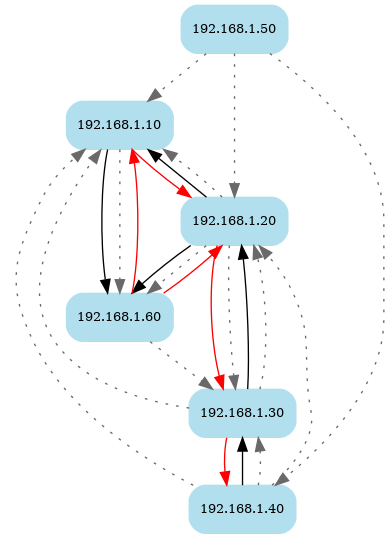
\includegraphics[scale=0.65]{chap6/network2.png}
	\caption{Simplified graph of the iTrust SWaT system network}
	\label{fig:6_network_SWaT}
\end{figure}

The graph clearly illustrates the structure of communications between the PLCs. Referring back to Table \ref{table:5_swat_ip_addresses}, which displays the IP address - PLC associations, we can observe that PLCs 1 through 4 communicate directly and sequentially with each other in a Request/Response communication pattern (represented by red and black arrows, respectively). Additionally, PLC6 communicates with both PLC1 and PLC2. On the other hand, the gray dotted arrows indicate communications for which we have knowledge of a response, but the corresponding request is unknown. For the purposes of our analysis strategy, we will not consider these communications within this context.

\bigskip
Based on our observations, the analysis strategy we will adopt involves considering sequential pairs of PLCs to effectively capture the relationships and implications between registers. Therefore, the PLC pairs we will focus on are PLC1-2, PLC2-3, and PLC3-4. 

\section{Reverse Engineering of the iTrust SWaT System}
\label{sec:6_reverse_SWaT}
Before we delve into the analysis, it is important to provide some preliminary remarks. 

\paragraph{Analysis structure}
\label{par:6_analysis_struture}
Firstly, the analysis will be structured as a schematic analysis due to space constraints, which prevent us from presenting the extensive inferences and reasoning regarding the system in full detail. However, the general procedure of the methodology and how to reason about the data obtained from the framework have already been demonstrated through examples on the PLC1 of the SWaT system in Chapter \ref{chap:proposal}. We encourage readers to refer to those examples for a more comprehensive understanding. In this analysis, our focus will be on illustrating the conjectures and properties that arise from the analysis, utilizing tables and the outputs generated during the analysis.

\paragraph{Defining subsystem time duration}
\label{par:6_subsystem_duration}
The second premise addresses the process of defining the subsystems to be analyzed, which were obtained during the pre-processing phase, during the merge phase of the individual datasets. Apart from the projection determined by the considered PLCs, a time-based selection of the analysis period has also been performed (see Section \ref{subsubsec:4_select_subsystem}). This selection spans a duration of 20,000 seconds, which is equivalent to approximately five and a half hours or roughly five system cycles. The analysis begins at 100,000 seconds, which corresponds to approximately 27 hours from the start of the available data. This deliberate selection aims to exclude the initial transient period during which the SWaT system is initialized. We believe that this time range is more than sufficient for accurately defining the characteristics of the SWaT system components.

\paragraph{Conventions}
\label{par:6_conventions}
The third premise introduces some conventions regarding the PLC registers that will be utilized during the analysis. These conventions aid in identifying the nature and function of the registers. Specifically:

\begin{enumerate}
	\item Registers containing \textit{discrete values}, such as binary or ternary values, are likely to represent \textbf{actuators}.
	
	\item Registers with \textit{continuous values} are likely to represent \textbf{measurements}.
	
	\item Actuators with three states are recognized as \textbf{valves}, while those with two states are considered \textbf{pumps}. The definitions of \textit{valve} and \textit{pump} in this context are arbitrary and primarily serve the purpose of distinguishing between the two types of registers.
	
	\item Measurements that encompass a broader spectrum of values, fluctuating between maximum and minimum thresholds, are commonly designated as \textbf{level sensors} utilized for tank monitoring. Conversely, Measurements characterized by a narrower range may serve other measurement purposes, such as \textbf{flow or pressure sensing}.
	
	\item Registers with a single constant value are recognized as either \textbf{relative setpoints} or \textbf{backup actuators}. The distinction is made based on the value contained in the register. Binary values or values corresponding to the states of the main actuators indicate backup actuators, while different values (e.g., 20, 40, 80, etc.) suggest the presence of relative setpoints.

	\item Registers with similar names, such as \texttt{P1\_LIT101} and \texttt{P3\_LIT301}, or \texttt{P2\_MV201} and \texttt{P3\_MV302}, indicate the same type of register, such as a valve, pump, level sensor, or other category.
\end{enumerate}

By following these conventions, it becomes easier to interpret and analyze the functionality of the PLC registers within the system.

\paragraph{About the Business Process Analysis}
\label{par:6_premesse_bpa}
In the end, the Business Process Analysis will focus solely on the physical process part. This is because the datasets of network traffic captures provided by iTrust for the year 2015 (as discussed in Section \ref{par:5_2015_net_dataset}) are \textbf{incomplete}. While communications related to measurements are present, those associated with actuators are entirely missing, as well as additional communications related to other system characteristics that we observed in the datasets of subsequent years. As a result, we were unable to incorporate the network event recognition component into our Business Process Analysis. To implement this component, we would require complete and overlapping network data, along with a clean physical process dataset not affected by system attacks. Unfortunately, none of the available iTrust datasets fulfill these criteria.

\subsection{Reverse Engineering of PLC1 and PLC2}
\label{subsec:6_P1P2_analysis}
The initial focus of analysis will be on the pair comprising PLC1 and PLC2. Let's delve into the main features of this subsystem by examining the outcomes obtained from applying the framework to it.

\subsubsection{Pre-processing - Preliminary Analysis}
\label{subsubsec:6_P1P2_preprocessing}

\paragraph{Measurements and Actuators Recognition} 
\label{par:6_P1P2_measures_actuators_recognition}
Listing \ref{lst:6_preproc_P1P2} shows the outcomes obtained from automatic recognition of likely measurements and actuators:

\begin{lstlisting}[language=bash, numbers=left, caption=Preliminary analysis outcomes for sensors and actuators of \texttt{PLC1-2}, label=lst:6_preproc_P1P2]
	Actuators: 
	P1_MV101 [0.0, 1.0, 2.0]
	P1_P101 [1.0, 2.0]
	P2_MV201 [0.0, 1.0, 2.0]
	P2_P203 [1.0, 2.0]
	P2_P205 [1.0, 2.0]
	
	Sensors: 
	P1_FIT101 {'max_lvl': 2.7, 'min_lvl': 0.0}
	P1_LIT101 {'max_lvl': 815.1, 'min_lvl': 489.6}
	P2_AIT201 {'max_lvl': 256.5, 'min_lvl': 252.9}
	P2_AIT202 {'max_lvl': 8.4, 'min_lvl': 8.3}
	P2_AIT203 {'max_lvl': 342.8, 'min_lvl': 320.0}
	P2_FIT201 {'max_lvl': 2.5, 'min_lvl': 0.0}
	
	Hardcoded setpoints or spare actuators: 
	P1_P102 [1.0]
	P2_P201 [1.0]
	P2_P202 [1.0]
	P2_P204 [1.0]
	P2_P206 [1.0]
\end{lstlisting}

Based on the results shown in Listing \ref{lst:6_preproc_P1P2}, the framework has recognized \texttt{P1\_MV101}, \texttt{P1\_P101}, \texttt{P2\_MV201}, \texttt{P2\_P203}, and \texttt{P2\_P205} as \textbf{likely actuators}. The actuators indicated by the \textit{Pxxx} string are binary actuators, meaning they have two states represented by the values 1 and 2. On the other hand, the actuators identified by the \textit{MVxxx} string are ternary actuators with three distinct states: 0, 1, and 2. According to the third premise of Section \ref{sec:6_reverse_SWaT}, for point 3, actuators denoted by the \textit{Pxxx} string will be classified as \textbf{pumps}, while those labeled with \textit{MVxxx} will be recognized as \textbf{valves}.

\bigskip
\texttt{P1\_FIT101}, \texttt{P1\_LIT101}, \texttt{P2\_AIT201}, \texttt{P2\_AIT202}, \texttt{P2\_AIT203}, and \texttt{P2\_FIT201} have been identified as \textbf{likely measurements}. Each measurement provides a specific range of values, spanning from a maximum to a minimum value. Based on the range of values reported by these measurements and according to the third premise of Section \ref{sec:6_reverse_SWaT}, for point 4, it is reasonable to infer that \texttt{P1\_LIT101} could potentially be a \textbf{level sensor for a tank}.

\bigskip
In addition, there are some registers that have been recognized as \textbf{hardcoded setpoints} or \textbf{spare actuators} due to their constant values. These registers share a resemblance to the previously identified pump registers. According to points 5 and 6 of the third premise in Section \ref{sec:6_reverse_SWaT}, it is reasonable to assume that these registers correspond to \textbf{spare actuators}. Furthermore, the fact that they have a constant value of 1 indicates that they might represent the \textbf{OFF state} of the pumps.

\paragraph{Actuator State Durations}
\label{par:6_P1P2_actuators_duration}
To gain a deeper understanding of the different states (0, 1, and 2) associated with valves \texttt{P1\_MV101} and \texttt{P2\_MV201}, we can analyze the duration of each state. Listing \ref{lst:6_preproc_P1P2_actuator_duration} provides information regarding the duration (in seconds) of states for these specific actuators:

\begin{lstlisting}[language=bash, numbers=left, caption=Time duration of the states of actuators \texttt{P1\_MV101} and \texttt{P1\_MV201} of PLC1-2, label=lst:6_preproc_P1P2_actuator_duration]
	Actuator state durations:
	P1_MV101 == 0.0
	9  9  10  9  9  10  9  9  10  9
	
	P1_MV101 == 1.0
	1174  1168  1182  1160  1172
	
	P1_MV101 == 2.0
	669  3019  3012  3000  2981
	
	P2_MV201 == 0.0
	8  8  8  9  9  8  9  9  9  9
	
	P2_MV201 == 1.0
	1057  1057  1045  1038  1039
	
	P2_MV201 == 2.0
	120  3135  3144  3127  3109
\end{lstlisting}

It is evident that the duration of \textbf{state 0 is relatively short}, averaging around 8-10 seconds, while the other states have much longer durations. This observation suggests that state 0 of a valve is a \textbf{transient state}, indicating a transitional phase within the valve cycle. However, without further information, it is currently not possible to determine the specific position of state 0 within the overall valve cycle.

\paragraph{Actuator State Changes}
\label{par:6_preproc_P1P2_actuator_state_changes}
Now that we have identified \texttt{P1\_LIT101} as the supposed tank, we can examine the trend of the tank level as the actuators change state. Listing \ref{lst:6_P1P2_preproc_changestate} provides information on the levels of the tank in correlation with the state changes of the \texttt{P1\_P101} pump:

\begin{lstlisting}[language=bash, numbers=left, caption=P1\_P101 state changes in relation to P1\_LIT101, label=lst:6_P1P2_preproc_changestate]
	P1_LIT101  P1_P101  prev_P1_P101
	 536.0356        1             2
	 533.3272        1             2
	 542.1591        1             2
	 534.8581        1             2
	 540.5890        1             2
	
	P1_LIT101  P1_P101  prev_P1_P101
	 813.0031        2             1
	 813.0031        2             1
	 811.8256        2             1
	 812.7283        2             1
	 813.3171        2             1
\end{lstlisting}

Based on the speculation that state 1 represents the OFF state of the pump and state 2 represents the ON state, we can analyze the data in Listing \ref{lst:6_P1P2_preproc_changestate}. When pump \texttt{P1\_P101} transitions from the ON state to the OFF state, the average level of \texttt{P1\_LIT101} is 535. On the other hand, when \texttt{P1\_P101} goes from the OFF state to the ON state, the average level of \texttt{P1\_LIT101} is 813. These values correspond to the \textbf{minimum and maximum relative setpoints} of \texttt{P1\_P101}, respectively. 

Based on this information, we can infer that pump \texttt{P1\_P101} is responsible for \textbf{emptying the tank}. Moreover, it can be extended to assume that a pump, in general, is responsible for \textbf{water outflow}.

\bigskip
Applying the same analysis to the data for valve \texttt{P1\_MV101}, which is not reported for conciseness, we can speculate that \texttt{P1\_MV101} is responsible for \textbf{filling the tank}. In this case, states 1 and 2 would represent the \textbf{OFF and ON states of the valve}, respectively. The relative setpoints of \texttt{P1\_MV101} are approximately 500 (minimum) and 800 (maximum).
By extending this analysis, we can speculate that a valve, such as \texttt{P1\_MV101}, is responsible for controlling the \textbf{water inflow}.

\bigskip
Regarding the elements controlled by PLC2 and the sensor \texttt{P1\_FIT101}, the analysis does not reveal the presence of another tank. Therefore, we cannot determine the exact role of sensors \texttt{P2\_AIT\textit{20x}}, \texttt{P1\_FIT101} and \texttt{P2\_FIT201} at this point.
However, there is a similarity observed between the relative setpoints of \texttt{P1\_P101} and those of \texttt{P2\_MV201}, \texttt{P2\_P203}, and \texttt{P2\_P205}. These registers exhibit very similar values during state changes, suggesting a potential relationship or similar control behavior between them.

\begin{comment}
\paragraph{Conjecture summarizing} We summarize in Table \ref{table:6_P1P2_summarize_preliminary} the conjectures made in this phase:

\bigskip
{	\footnotesize
	\begin{longtable}[l]{p{0.05\textwidth} p{0.45\textwidth} p{0.45\textwidth}}
		\hline
		\textbf{\#} & \textbf{Statement} & \textbf{Reason} \\
		\hline
		
		C1 & \texttt{P1\_LIT101}, \texttt{P1\_FIT101}, \texttt{P2\_FIT201}, \texttt{P2\_AIT201}, \texttt{P2\_AIT202}, \texttt{P2\_AIT203} are \textbf{measurements}. & Registers contain continuous numerical values.\\
		\hline
		
		C2 & \texttt{P1\_LIT101} is identified as the \textbf{level sensor} specifically associated with a \textbf{tank} & Sensor has a wide range of values (minimum 489, maximum value of 815).\\
		\hline
		
		C3 & \texttt{P1\_MV101}, \texttt{P1\_P101}, \texttt{P2\_MV201}, \texttt{P2\_P203} and \texttt{P2\_P205} are \textbf{actuators}. & Registers contain discrete numerical values.\\
		\hline
		
		C4 & \texttt{P1\_MV101} and \texttt{P2\_MV201} assume three distinct states, represented by the values 0, 1, and 2. They can be identified as \textbf{valves}.& Observation derived from output and point 3 of the third premise in Section \ref{par:6_conventions}\\
		\hline
		
		C5 & \texttt{P1\_P101}, \texttt{P2\_P203} and \texttt{P2\_P205} assume two distinct states, represented by the values 1, and 2. They can be identified as \textbf{pumps}. & Observation derived from output and point 3 of the third premise in Section \ref{par:6_conventions}\\
		\hline
		
		C6 & \texttt{P1\_102}, \texttt{P2\_P201}, \texttt{P2\_P202}, \texttt{P2\_P204} and \texttt{P2\_P206} are \textbf{spare actuators}. & Registers contain constant numerical values.\\
		\hline 
		
		C7 & A spare actuator in state 1 is considered to be \textbf{OFF}. & Speculation on the actuator states.\\
		\hline
		
		C8 & The state 0 of a valve is a \textbf{transient state}. & The duration of state 0 is only a few seconds. However, the subsequent states, have a significantly longer duration.\\
		\hline
		
		C9 & State 1 of the pump \texttt{P1\_P101} corresponds to the \textbf{OFF state} of the actuator; state 2 of \texttt{P1\_P101} corresponds to the \textbf{ON state} of the actuator. & Derived from Conjecture C7.\\ 
		\hline
		
		C10 & The \textit{relative setpoints} of \texttt{P1\_P101} are approximately 535 (minimum) when state change to OFF and approximately 813 (maximum) when state change to ON. & Observation derived from output\\
		\hline
		
		C11 & \texttt{P1\_P101} is responsible for \textbf{emptying the tank} represented by \texttt{P1\_LIT101}. & Derived from Conjecture C9 and C10 \\
		\hline
		
		C12 & Pumps are responsible for \textbf{water outflow}. & Corollary to Conjecture C11\\
		\hline	
		
		C13 & State 1 of the valve \texttt{P1\_MV101} corresponds to the \textbf{OFF state} of the actuator; state 2 of \texttt{P1\_MV101} corresponds to the \textbf{ON state} of the actuator. & Derived from Conjecture C7.\\
		\hline
		
		C14 & The \textit{relative setpoints} of \texttt{P1\_MV101} are approximately 500 (minimum) when state change to 2 and approximately 800 (maximum) when state change to 1. & Observation derived from output\\
		\hline
		
		C15 & \texttt{P1\_MV101} is responsible for \textbf{filling the tank} represented by \texttt{P1\_LIT101}. & Derived from Conjecture C13 and C14 \\
		\hline
		
		C16 & Valves are responsible for \textbf{water intake}. & Corollary to Conjecture C15\\
		\hline
		
	\caption{}
	\label{table:6_P1P2_summarize_preliminary}
	\end{longtable}
}
\end{comment}

\subsubsection{Graphs and Statistical Analysis}
\label{subsubsec:6_P1P2_graphs}

\begin{figure}[ht]
	\centering
	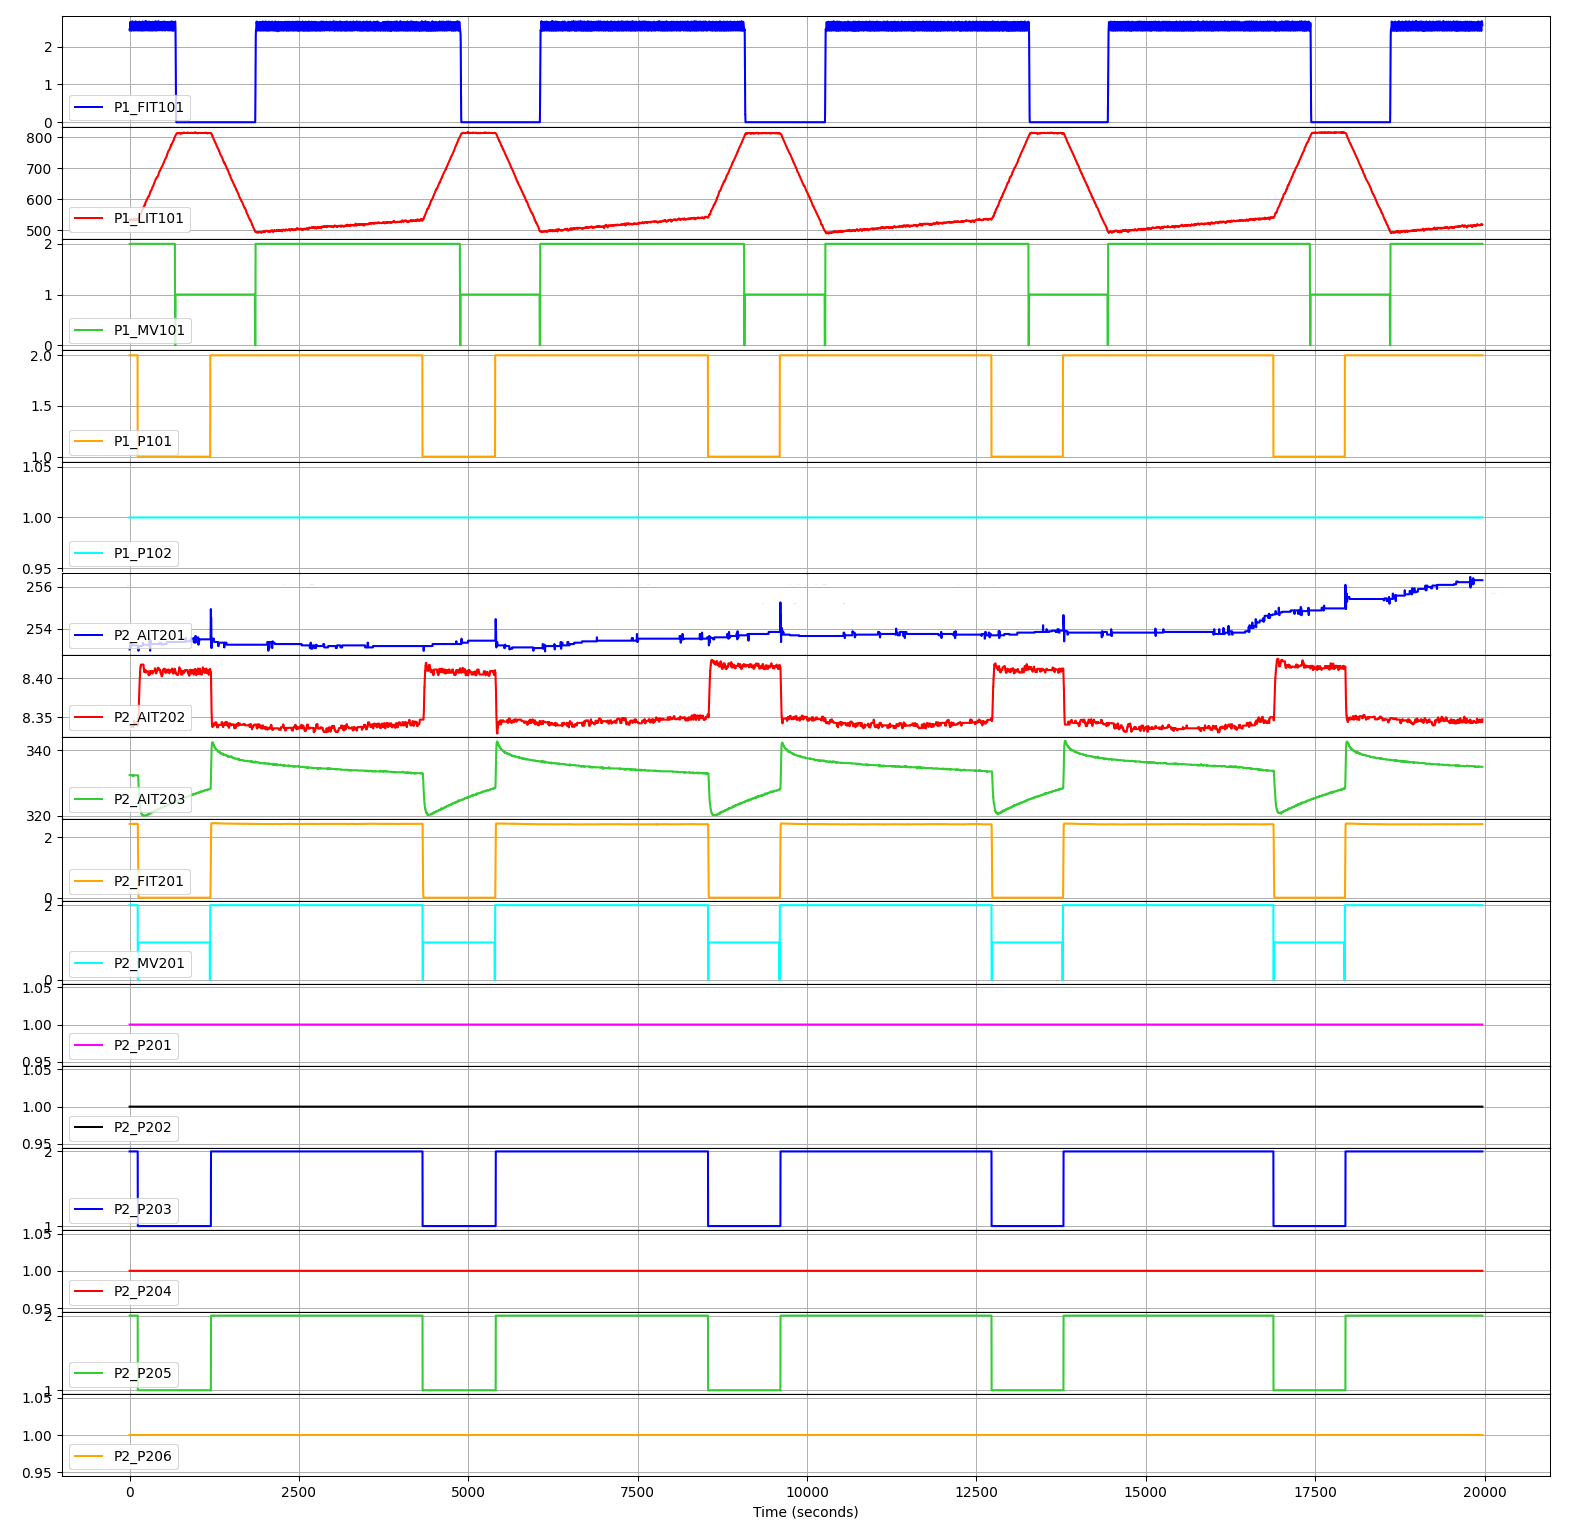
\includegraphics[scale=0.34]{chap6/P1P2_1a.png}
	\caption{Chart of PLC1-2 registers}
	\label{fig:6_P1P2_graph_full}
\end{figure}

Figure \ref{fig:6_P1P2_graph_full} illustrates the graphical representation of the registers in PLC1-2 and their respective trends.

The image provides additional support to the conjectures made during the preliminary analysis regarding the spare actuators. Furthermore, it is evident from the graphs that these spare actuators \textbf{do not appear to influence the trend} of any of the measurements. Therefore, based on this observation, we can confidently exclude these registers from further graphical analysis.

\bigskip
Figure \ref{fig:6_P1P2_graph_full_nospare} shows a clearer representation of the subsystem after removing the spare actuators.

\begin{figure}[ht]
	\centering
	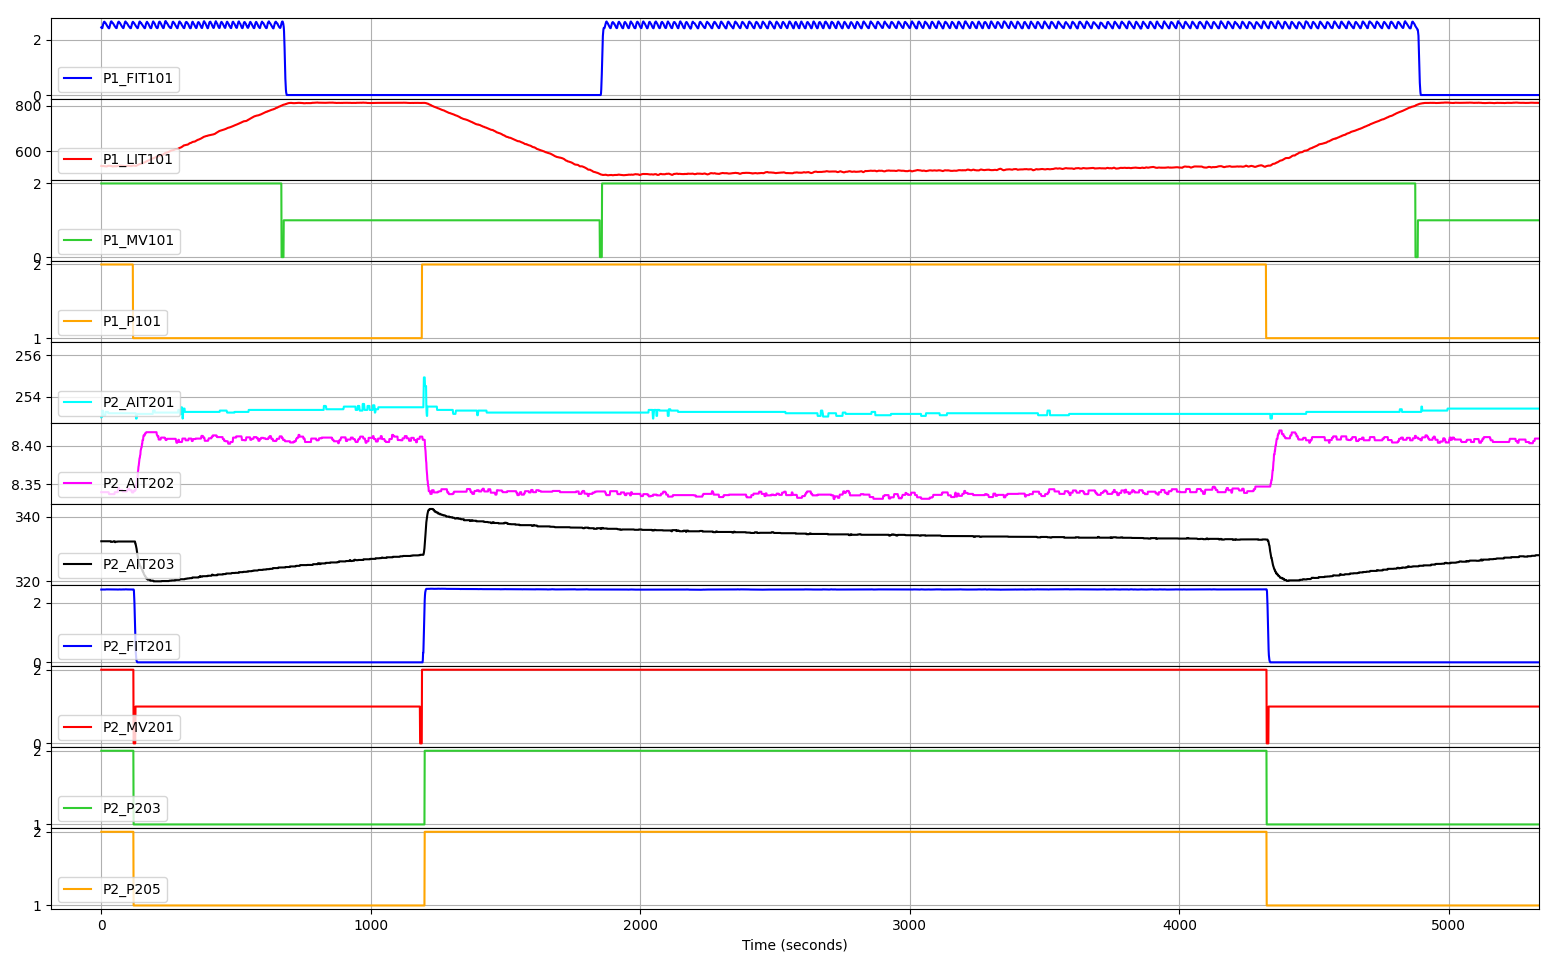
\includegraphics[scale=0.35]{chap6/P1P2_5.png}
	\caption{Chart of PLC1-2 registers without spare actuators (particular)}
	\label{fig:6_P1P2_graph_full_nospare}
\end{figure}

Figure %\ref{fig:6_P1P2_graph_full_nospare} 
provides furthermore additional insights that allow us to speculate on aspects that remained unexplained during the preliminary analysis. The most prominent aspect that stands out is the relationship between the level behavior of \texttt{P1\_LIT101} and the states of \texttt{P1\_P101} and \texttt{P1\_MV101}. It becomes evident that these two actuators \textbf{are \textit{not} mutually exclusive}, and when they are both in the ON state, the growth of the tank level is slow. However, as soon as {P1\_P101} switches to the OFF state, the tank level starts to increase at a faster rate. Conversely, when \texttt{P1\_MV101} switches to the OFF state, the tank level decreases. During periods when both actuators are in the OFF state, there is a \textit{plateau} where the tank level remains relatively stable.

\bigskip
Furthermore, we observe a relationship between \texttt{P1\_FIT101} and the trend of \texttt{P1\_MV101}. When the valve is in the off state, \texttt{P1\_FIT101} registers a value of 0, whereas it registers a value greater than 2 when the valve is open. This suggests that \texttt{P1\_FIT101} could be a \textbf{sensor associated with the flow} of water entering the tank, which is represented by \texttt{P1\_LIT101}. By drawing an analogy with its name, it is plausible to consider \texttt{P2\_FIT201} as another flow sensor.

\bigskip
Another intriguing aspect that arises from examining the graphs in Figure \ref{fig:6_P1P2_graph_full} and Figure \ref{fig:6_P1P2_graph_full_nospare} is the \textbf{non-cyclic pattern} observed in the \texttt{P2\_AIT201} measurement. Instead of exhibiting a cyclical trend, it follows a linear pattern. Furthermore, considering the narrow range of values associated with this measurement, it is reasonable to speculate that \texttt{P2\_AIT201} may be associated with a \textbf{sensor that measures a specific property of the water}.

The limited range of values observed in \texttt{P2\_AIT202} also raises the possibility that it functions as a sensor for a particular water characteristic, despite exhibiting a cyclic pattern. As for \texttt{P2\_AIT203}, its role remains undefined, although it also displays a cyclic trend. This trend, along with that of \texttt{P2\_AIT202}, does not appear to be related to the behavior of the valves (which rules out the possibility of it being related to a tank), but rather to that of the pumps. Consequently, it is imperative to conduct further investigations into these aspects.

\bigskip
By examining the trend of valve \texttt{P2\_MV201}, an additional speculation can be made. It appears to be independent of the trends observed in any of the measurements within this subsystem. Based on previous conjectures regarding the role of valves and considering the duration of its ON and OFF states, it is possible that \texttt{P2\_MV201} is responsible for \textbf{filling a tank that is not part of this particular subsystem}. Once again, a thorough investigation is necessary to confirm this hypothesis.

\begin{comment}
\paragraph{Conjecture summarizing}
We summarize in Table \ref{table:6_P1P2_summarize_graphs} the conjectures made in this phase:

\bigskip
{	\footnotesize
	\begin{longtable}[l]{p{0.05\textwidth} p{0.45\textwidth} p{0.45\textwidth}}
		\hline
		\textbf{\#} & \textbf{Statement} & \textbf{Reason} \\
		\hline
		
		C17 & Valve \texttt{P1\_MV101} and pump \texttt{P1\_P101} are \textit{not} mutual exclusive. & Observation derived from the plot.The two actuators can assume the same state in the same time period.\\
		\hline
		
		C18 & When valve \texttt{P1\_MV101} and pump \texttt{P1\_P101} are both in the ON state, the tank level grows slowly. & Observation derived from the plot\\
		\hline
		
		C19 & When valve \texttt{P1\_MV101} is in the ON state and pump \texttt{P1\_P101} switches to the OFF state, \texttt{P1\_LIT101} level increase faster. & Observation derived from the plot\\
		\hline
		
		C20 & When valve \texttt{P1\_MV101} switches to the OFF state and pump \texttt{P1\_P101} is the ON state, \texttt{P1\_LIT101} level decreases. & Observation derived from the plot\\
		\hline
		
		C21 & When valve \texttt{P1\_MV101} and pump \texttt{P1\_P101} are both in the ON state, \texttt{P1\_LIT101} level is stable. & Observation derived from the plot\\
		\hline
		
		C22 & The trend of \texttt{P1\_FIT101} follows the trend of \texttt{P1\_MV101} & \texttt{P1\_FIT101} takes a value of 0 when the valve \texttt{P1\_MV101} is OFF, and positive values (> 2) when the valve is ON.\\
		\hline
		
		C23 & \texttt{P1\_FIT101} is a \textbf{flow sensor} related to the inlet water flow at \texttt{P1\_LIT101}. & Corollary to Conjecture C17\\ 
		\hline
		
		C24 & \texttt{P2\_FIT201} is also a likely \textbf{flow sensor}. & By analogy with \texttt{P1\_FIT101} (point 6 of the third premise in Section \ref{par:6_conventions})\\ 
		\hline
		
		C25 & There is a correlation between the trend of \texttt{P1\_P101} and the trend of \texttt{P2\_MV201}. & Observation derived from the plot\\ 
		\hline
		
		C26 & \texttt{P2\_MV201} is responsible for \textbf{filling a tank} that is \textit{not} part of this subsystem. & Sensors \texttt{P2\_AIT202} and \texttt{P2\_AIT203} do not exhibit an increasing trend when the valve is ON, and there is no apparent correspondence between the trend of the valve and the trend of \texttt{P1\_LIT101}.\\ 
		\hline
		
		C27 & \texttt{P2\_AIT201} is a sensor that measures \textbf{some property of the water}. & Measurement does not show a cyclic pattern in its measurements.\\
		\hline
		
		C28 & \texttt{P2\_AIT202} is a sensor that measures \textbf{some property of the water}. & Very narrow range between maximum and minimum values (point 4 of the third premise in Section \ref{par:6_conventions})\\
		\hline
		
		C29 & The trend of \texttt{P2\_AIT202} and \texttt{P2\_AIT203} follows the trend of \texttt{P2\_P20x} pumps & Observation derived from the plot\\ 
		\hline
		
	\caption{}
	\label{table:6_P1P2_summarize_graphs}
	\end{longtable}
}
\end{comment}
		
\subsubsection{Invariant Inference and Analysis}
\label{subsubsec:6_P1P2_invariants}
Through the process of \textit{invariant analysis}, we aim to discover new information about the system and determine whether the conjectures made in the previous steps are supported by the data obtained from the Daikon analysis.

\paragraph{General Invariants}
We will begin this phase by analyzing the general invariants (see Section 4.2.5.1.). Listing \ref{lst:6_preproc_P1P2_general_invariants} presents a selection of these invariants:

\begin{lstlisting}[language=bash, numbers=left, caption=General Invariants for PLC1-2, label=lst:6_preproc_P1P2_general_invariants]
	P2_P206 == P2_P204 == P2_P202 == P2_P201 == P1_P102 == 1.0
	P2_P205 == P2_P203
	max_P1_LIT101 == 816.0
	min_P1_LIT101 == 489.0
	max_P2_AIT201 == 257.0
	min_P2_AIT201 == 252.0
	max_P2_AIT202 == 9.0
	min_P2_AIT202 == 8.0
	max_P2_AIT203 == 343.0
	min_P2_AIT203 == 320.0
\end{lstlisting}

The invariant mentioned on line 2 is particularly significant: it states that \texttt{P2\_P203} and \texttt{P2\_P205} always have the same values. While this information was somewhat apparent in the previous steps, it becomes more apparent and evident in this analysis. This observation leads us to speculate that the two pumps, \texttt{P2\_P203} and \texttt{P2\_P205}, \textbf{are related to each other} in some way. The other invariants provided in this section further reinforce the hypotheses about the spare actuators.

\paragraph{Analysis on Single Actuator States}
\label{par:6_P1P2_single_act_states}
We proceed with the examination of the invariants derived from the \textit{first of the two semi-automatic analysis} discussed in Section \ref{par:4_single_actuator_states_analysis}. Specifically, we will focus on the analysis concerning the states of individual actuators in relation to a specific measurement, which in our case pertains to the tank represented by \texttt{P1\_LIT101}. For illustrative purposes, let's consider states 1 and 2 (OFF e ON respectively) of valve \texttt{P1\_MV101} as an example (we will disregard state 0 as it is considered transient). The conditional invariants pertinent to this scenario can be found in Listing \ref{lst:6_preproc_P1P2_conditional_invariants}.

\begin{lstlisting}[language=bash, numbers=left, caption=Conditional Invariants for states 1 and 2 of \texttt{P1\_MV101}, label=lst:6_preproc_P1P2_conditional_invariants]
	===========================
	P1_MV101 == 1.0 && P1_LIT101 < max_P1_LIT101 - 16 && P1_LIT101 > min_P1_LIT101 + 15 
	===========================
	...
	P2_P205 == P2_P203 == P2_MV201 == P1_P101 == 2.0
	P1_FIT101 == 0.0
	slope_P1_LIT101 == -1.0
	P2_FIT201 > P1_FIT101
	P2_FIT201 > P1_MV101
	P2_FIT201 > P1_P101
	...
	
	===========================
	P1_MV101 == 2.0 && P1_LIT101 < max_P1_LIT101 - 16 && P1_LIT101 > min_P1_LIT101 + 15 
	===========================
	slope_P1_LIT101 == P1_P102
	P1_FIT101 > P1_MV101
	...
	P1_MV101 >= P1_P101
	P1_MV101 >= P2_MV201
	P1_MV101 >= P2_P203
	P2_P203 >= P1_P101
	...
\end{lstlisting}

To prevent transient periods caused by water flow stabilization when the actuators change state, a condition is imposed on the level of \texttt{P1\_LIT101}. However, this condition may result in an incomplete understanding of the system's behavior. To address this, a manual refinement of the analysis is required, utilizing the \texttt{runDaikon.py} script as outlined in Section \ref{par:4_refining_analysis}.

\bigskip
Based on the analysis, the following observations can be made when the valve is in the OFF state:

\begin{itemize}
	\item The slope of \texttt{P1\_LIT101}, denoted as \texttt{slope\_P1\_LIT101}, is negative (line 7). This indicates a \textbf{downward trend} in the tank level, as we have seen in Section \ref{par:6_preproc_P1P2_actuator_state_changes}.
	\item \texttt{P1\_P101} is in state 2, or ON (line 5).
	\item \texttt{P1\_FIT101} is zero (line 6).
	\item \texttt{P2\_FIT201} has a value greater than 2 (line 10).
\end{itemize}

\noindent On the other hand, when the valve is in the ON state:

\begin{itemize}
	\item \texttt{slope\_P1\_LIT101} is positive (line 16). This indicates an \textbf{upward trend} in the tank level, as we have seen in Section \ref{par:6_preproc_P1P2_actuator_state_changes}.
	\item \texttt{P1\_FIT101} assumes a value greater than 2. The combination of this finding, along with the previous one regarding the same register, strengthens the hypothesis that this is indeed a flow sensor.
	\item \texttt{P1\_P101} can be in either the ON or OFF state, as we have seen in Section \ref{subsubsec:6_P2P3_graphs}.
\end{itemize}

When conducting a manual analysis using the \texttt{runDaikon.py} script on tank levels that fall outside the range defined by the previous condition, it does not yield useful slope information. This situation can occur because, despite the noise attenuation applied to the tank level sensor data, if there is even a single cycle in the system where the calculated slope deviates from the expected outcome, it can adversely affect the entire Daikon analysis. Figure \ref{fig:6_P1P2_slope_fail} shows this behavior.

\begin{figure}[ht]
	\centering
	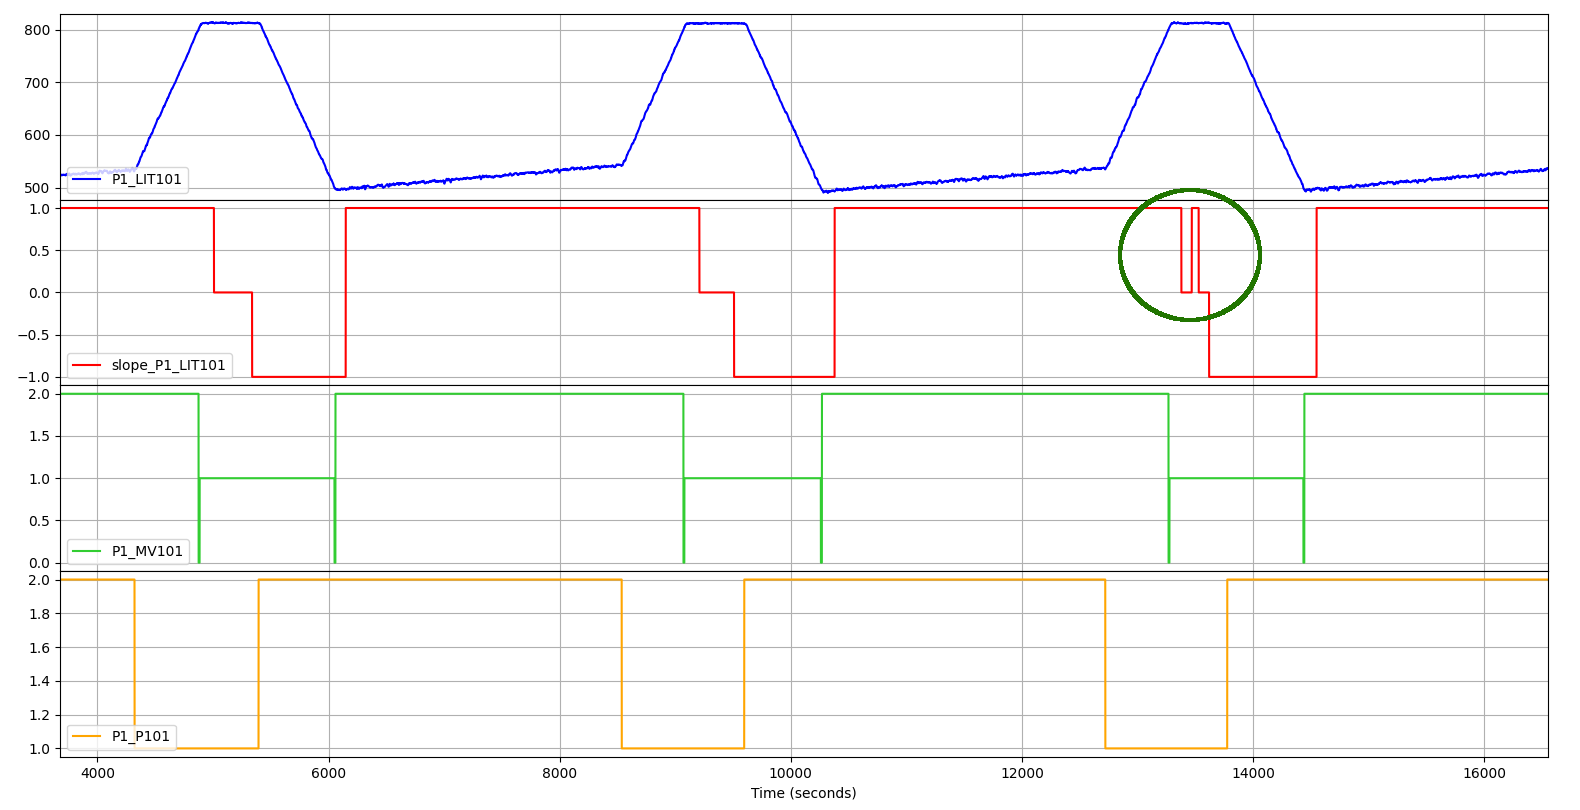
\includegraphics[scale=0.35]{chap6/P1P2_slope_error.png}
	\caption{Slope calculation anomaly (in the circle)}
	\label{fig:6_P1P2_slope_fail}
\end{figure}

\paragraph{Analysis of the Current System Configuration}
\label{par:6_P1P2_current_system_conf}
We conclude our analysis of invariants by considering the \textit{second semi-automatic analysis} outlined in Section \ref{par:4_current_system_config_analysis}, which focuses on the effective states of the system. Due to the comprehensive nature of this analysis, we will not provide a detailed report of the outputs to maintain brevity. However, this analysis confirms the findings observed in the analysis of individual actuator states. Additionally, one crucial piece of information becomes apparent for future steps: the changing state of the actuators controlled by PLC2 \textbf{do \textit{not} impact the behavior of the tank} controlled by PLC1. Indeed, it is sufficient to examine the invariant pertaining to the slope of the tank to verify this observation.

\begin{comment}
\paragraph{Conjecture summarizing}
We summarize in Table \ref{table:6_P1P2_summarize_invariants} the conjectures made in this phase:

\bigskip
{	\footnotesize
	\begin{longtable}[l]{p{0.05\textwidth} p{0.45\textwidth} p{0.45\textwidth}}
		\hline
		\textbf{\#} & \textbf{Statement} & \textbf{Reason} \\
		\hline
		
		C30 & \texttt{P2\_P203} and \texttt{P2\_P205} always have the same values. & Observation derived from the general invariants.\\
		\hline
		
		C31 & Actuators controlled by PLC2 do \textit{not} impact the behavior of \texttt{P1\_LIT101}. & Observation derived from the analysis of the current system configuration.\\
		\hline
		
	\caption{}
	\label{table:6_P1P2_summarize_invariants}
	\end{longtable}
}
\end{comment}

\subsubsection{Business Process Mining and Analysis}
\label{subsubsec:6_P1P2_bpa}
As explained in Section \ref{subsub:4_proc_minining_phy}, the \textit{process mining phase} applied to the physical system provides us with an immediate understanding of the system cycle and the chronological sequence of states. It enables us to determine the duration of time the system remains in a particular state and at what relative setpoint the state transition occurs concerning the reference measure. Furthermore, we can analyze the trend of this measure within each state. Additionally, we can examine the relative setpoints of other measurements to identify any connections between changes in system state and these values. 

\bigskip
Given that we have already identified the likely measurement representing the tank and the corresponding actuators that control its behavior, an activity diagram can be generated as depicted in Figure \ref{fig:6_P1P2_process_mining}.

\begin{figure}[ht]
	\centering
	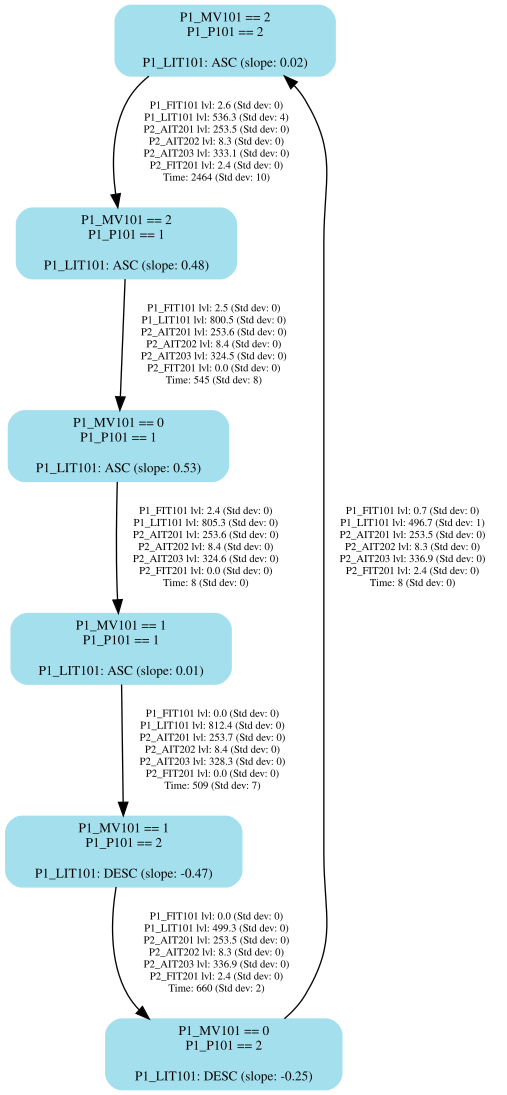
\includegraphics[scale=0.35]{chap6/business_process_P1P2.png}
	\caption{Activity diagram for PLC1-2}
	\label{fig:6_P1P2_process_mining}
\end{figure}

\bigskip
The activity diagram allows for easy interpretation of the tank level trend and slope within different states. The states where the valve has a value of 0 can be disregarded due to their short duration. Similar to the graphical analysis, there is an observed change in slope during the increasing trend of the tank level between the states \texttt{[P1\_MV101 == 2, P1\_P101 == 2]} and \texttt{[P1\_MV101 == 2, P1\_P101 == 1]}, where the slope changes from 0.02 to 0.48.

Additionally, the timing analysis on the edges reveals that the tank takes longer to fill than to empty, and the system remains in the \texttt{[P1\_MV101 == 1, P1\_P101 == 1]} state for approximately 8 minutes (509 seconds).

\bigskip
Regarding the state \texttt{[P1\_MV101 == 1, P1\_P101 == 1]}, there appears to be a discrepancy between the trend of the tank level as reported in the activity diagram and the conjectures made in the previous phases of the analysis. The activity diagram correctly depicts an increasing trend in the tank level between the end of the state \texttt{[P1\_MV101 == 2, P1\_P101 == 1]} and the end of the state \texttt{[P1\_MV101 == 1, P1\_P101 == 1]}. However, the discrepancy arises due to the fact that the interruption of flow during the valve state change from state ON to state OFF is not immediate, mainly due to the presence of the transient state 0. Additionally, water continues to flow within the piping towards the tank for a short duration even after the valve is closed. After this period, which usually lasts a few seconds, the tank level stabilizes, and there is no further inflow or outflow of water. 

By adjusting the tolerance parameter \texttt{-t} in the \texttt{processMining.py} script, it is possible to obtain accurate data regarding the behavior of the state corresponding to the \textit{plateau} observed in the graphical analysis.

\bigskip
The data presented on the arcs in the activity diagram represents the measurement values relative to the time of system state changes, specifically the relative setpoints. These values are calculated based on the average data collected in each cycle. By analyzing this data, we can observe the tank level values at which the system undergoes configuration changes and how the trend of the tank level changes accordingly. Specifically, we can see that the trend transitions from ascending to stable at a tank level value of 800, from stable to descending at approximately 812, and from descending back to ascending at around 499. The change in the speed of tank filling occurs at approximately 535.

\bigskip
Furthermore, the data provides additional support for the hypothesis that the measurements associated with registers \texttt{P2\_AIT20x} are not influenced by the tank's trends.

\subsubsection{Properties}
\label{subsubsec:6_P1P2_summary_table}
From the conjectures derived from the four phases of the analysis we will derive the properties of the subsystem we are studying, which will be placed within a \textbf{summary table}. This table contains an integer identifying the property, the statement of the property itself, and from which of the four phases it was derived.

\bigskip
{\footnotesize
	\begin{longtable}[l]{p{0.05\textwidth} p{0.57\textwidth} p{0.30\textwidth}}
		\hline
		\textbf{\#} & \textbf{Statement} & \textbf{Derived from} \\
		\hline
		
		P1 & The registers \texttt{P1\_LIT101}, \texttt{P1\_FIT101}, \texttt{P2\_AIT201}, \texttt{P2\_AIT202}, \texttt{P2\_AIT203}, and \texttt{P2\_FIT201} are considered measurements. & Preliminary Analysis\newline Graphical Analysis\\
		\hline
		
		P2 & The registers \texttt{P1\_MV101}, \texttt{P1\_P101}, \texttt{P2\_MV201}, \texttt{P2\_P203}, and \texttt{P2\_P205} are considered actuators. & Preliminary Analysis\newline Graphical Analysis\\
		\hline
		
		P3 & The actuators that contain the substring "MVxxx" are considered to be three-state actuators. For simplicity, we refer to them as valves. & Preliminary Analysis\\
		\hline
		
		P4 & The state 0 of these valves represents a transient state that occurs during the transition between state 1 (OFF) and state 2 (ON). & Preliminary Analysis\newline Graphical Analysis\\
		\hline
		
		P5 & The actuators that contain the substring "Pxxx" are considered to be binary actuators. For simplicity, we refer to them as pumps. & Preliminary Analysis \\
		\hline
		
		P6 & The registers \texttt{P1\_P102}, \texttt{P2\_P201}, \texttt{P2\_P202}, \texttt{P2\_P204}, and \texttt{P2\_P206} are considered spare actuators. They do \textit{not} influence the trend of any measurements and they are considered in the OFF state. & Preliminary Analysis\newline Graphical Analysis\newline Invariant Analysis \\
		\hline
		
		P7 & \texttt{P1\_LIT101} represents the level sensor of the tank controlled by PLC1. & Preliminary Analysis\newline Graphical Analysis\\
		\hline
		
		P8 & \texttt{P1\_MV101} and \texttt{P1\_P101} are the actuators responsible for the level behavior of the water contained in the tank. & Graphical Analysis\newline Invariant Analysis\newline Business Process\\
		\hline
		
		P9 & \texttt{P1\_MV101} is responsible for filling the tank. \texttt{P1\_P101} is responsible for emptying the tank. & Graphical Analysis\newline Invariant Analysis\\
		\hline
		
		P10 & Valve are responsible for water inflow. Pumps responsible for water outflow. & Preliminary Analysis\newline Graphical Analysis\newline Invariant Analysis\\
		\hline
		
		P11 & The rate of tank level growth is slow when both \texttt{P1\_MV101} and \texttt{P1\_P101} are in the ON state. The growth speed increases when \texttt{P1\_P101} transitions to the OFF state. & Graphical Analysis\newline Business Process\\
		\hline
		
		P12 & The tank level decreases when \texttt{P1\_MV101} is in the OFF state and \texttt{P1\_P101} is in the ON state. & Graphical Analysis\newline Invariant Analysis\\
		\hline
		
		P13 & The tank level remains (relatively) stable when both \texttt{P1\_MV101} and \texttt{P1\_P101} are in the OFF state. & Graphical Analysis\newline Business Process\\
		\hline
		
		P14 & The trend of the tank level transitions from ascending to stable when the level reaches approximately 800. It shifts from stable to descending when the level averages around 812. It changes from descending back to ascending when the level reaches about 500. The speed of tank filling increases noticeably at around 535. & Business Process \\
		\hline
		
		P15 & Absolute setpoints are 800, 812, 500 and 535. & Business Process \\
		\hline
		
		P16 & \texttt{P1\_FIT101} serves as a flow sensor to measure the inflow of water into the tank. & Graphical Analysis\newline Invariant Analysis\newline Business Process \\
		\hline
		
		P17 & None of the actuators connected to PLC2 have an impact on the level of the tank controlled by PLC1. & Graphical Analysis\newline Invariant Analysis\newline Business Process \\
		\hline
		
		P18 & None of the measurements connected to PLC2 represent a tank. & Preliminary Analysis\newline Graphical Analysis\\
		\hline
		
		P19 & \texttt{P2\_AIT201} does not exhibit a cyclic trend. & Graphical Analysis\\
		\hline
		
		P20 & Both \texttt{P2\_AIT201} and \texttt{P2\_AIT202} serve as sensors for measuring certain properties of the water. & Preliminary Analysis\newline Graphical Analysis\\
		\hline
		
		P21 & The behavior and trend of \texttt{P2\_AIT202} and \texttt{P2\_AIT203} are directly associated with the operation of the pump. & Graphical Analysis\newline Invariant Analysis\\
		
		\caption{Properties of the PLC1-2 subsystem}
		\label{table:6_P1P2_summarize_properties}
	\end{longtable}
}

\vfill

\subsection{Reverse Engineering of PLC2 and PLC3}
\label{subsec:6_P2P3_analysis}

\subsubsection{Pre-processing}
\label{subsubsec:6_P2P3_preprocessing}

\subsubsection{Graphs and Statistical Analysis}
\label{subsubsec:6_P2P3_graphs}

\subsubsection{Invariant Inference and Analysis}
\label{subsubsec:6_P2P3_invariants}

\subsubsection{Business Process Mining and Analysis}
\label{subsubsec:6_P2P3_bpa}

\subsection{Reverse Engineering of PLC3 and PLC4}
\label{subsec:6_P3P4_analysis}

\subsubsection{Pre-processing}
\label{subsubsec:6_P3P4_preprocessing}

\subsubsection{Graphs and Statistical Analysis}
\label{subsubsec:6_P3P4_graphs}

\subsubsection{Invariant Inference and Analysis}
\label{subsubsec:6_P3P4_invariants}

\subsubsection{Business Process Mining and Analysis}
\label{subsubsec:6_P3P4_bpa}

\vfill
\nolinenumbers